\documentclass[tikz, border=4pt]{standalone}
\usepackage{tikz}
\usepackage{tikz-cd}
\begin{document}
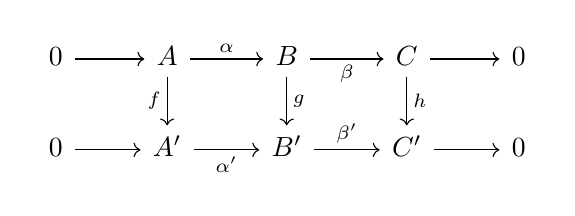
\begin{tikzpicture}[x=1cm, y=1cm]
  \node at (3.18,-0.9) {\pgfinterruptpicture%
  \begin{tikzcd}
    0 \arrow[r] & A \arrow[r, "\alpha"] \arrow[d, "f"'] & B \arrow[r, "\beta"'] \arrow[d, "g"] & C \arrow[r] \arrow[d, "h"] & 0 \\
    0 \arrow[r] & A' \arrow[r, "\alpha'"'] & B' \arrow[r, "\beta'"] & C' \arrow[r] & 0
  \end{tikzcd}%
  \endpgfinterruptpicture};
\end{tikzpicture}
\end{document}
